\documentclass[11pt,a4paper]{article}
\usepackage[T1]{fontenc}
\usepackage[utf8]{inputenc}
\usepackage{lmodern}
\usepackage{amsmath,amssymb,amsthm,mathtools}
\usepackage{geometry}
\geometry{margin=2.6cm}
\usepackage{booktabs,tabularx,array}
\usepackage{enumitem}
\usepackage[dvipsnames]{xcolor}
\usepackage{tikz}
\usetikzlibrary{arrows.meta}
\usepackage[hidelinks]{hyperref}
\hypersetup{pdftitle={Reading the IUT dispute through indexed identifications},pdfauthor={Toshihisa Urahigashi}}
\setlist{itemsep=2pt,topsep=4pt}
\raggedbottom
\emergencystretch=3em

\newcommand{\R}{\mathbb{R}}
\newcommand{\Rp}{\mathbb{R}_{>0}}
\newcommand{\Z}{\mathbb{Z}}
\newcommand{\qq}{\underline{\underline{q}}{}}
\newcommand{\Th}{\underline{\underline{\Theta}}{}}
\newcommand{\Gseg}{\Gamma_{\mathrm{seg}}}
\newcommand{\Gtwo}{\Gamma_{\mathrm{two}}}
\newcommand{\Gloop}{\Gamma_{\mathrm{loop}}}
\newcommand{\Guni}{\Gamma_{\mathrm{uni}}}
\newcommand{\id}{\mathrm{id}}

% labels
\newcommand{\lab}[2]{{\upshape\fcolorbox{#1}{#1!8}{\scriptsize\sffamily\bfseries\textcolor{#1}{#2}}}}
\newcommand{\tagS}{\lab{blue}{S}}
\newcommand{\tagP}{\lab{ForestGreen}{P}}
\newcommand{\tagR}{\lab{teal}{R}}
\newcommand{\tagN}{\lab{BrickRed}{N}}
\newcommand{\tagH}{\lab{BurntOrange}{H}}
\newcommand{\known}[1]{\par\noindent{\footnotesize\upshape Known mathematics: #1}\par\smallskip}
\newcommand{\companion}[1]{\par{\footnotesize Companion paper: #1}\par}
\newcommand{\q}[1]{``#1''}
\newcommand{\srcquote}[2]{\begin{quote}\small\tagS\ #1\par\nopagebreak\hfill{\footnotesize #2}\end{quote}}

\theoremstyle{plain}
\newtheorem{theorem}{Theorem}[section]
\newtheorem{proposition}[theorem]{Proposition}
\newtheorem{corollary}[theorem]{Corollary}
\theoremstyle{definition}
\newtheorem{definition}[theorem]{Definition}
\newtheorem{setup}[theorem]{Setup}
\newtheorem{example}[theorem]{Example}
\newtheorem{exercise}{Exercise}
\theoremstyle{remark}
\newtheorem{remark}[theorem]{Remark}

\title{Reading the IUT dispute through indexed identifications:\\ an educational model in undergraduate mathematics}
\author{Toshihisa Urahigashi\\\small ORCID 0009-0004-0460-6242\\\small\texttt{123026.urahigashi.toshihisa@gmail.com}}
\date{Version 1.0.0, 4 November 2026\\\small\href{https://doi.org/10.5281/zenodo.23931346}{doi:10.5281/zenodo.23931346}}

\begin{document}
\maketitle

\begin{abstract}
The dispute between Scholze--Stix and Mochizuki over Corollary~3.12 of inter-universal Teichm\"uller theory (IUT)~III
has been described in words: are isomorphic copies to be identified or not? This note gives an educational model that
states the \emph{shape} of the dispute precisely using only undergraduate mathematics---sets and maps, multiplication of
positive real numbers, graphs, and inequalities. Instead of the equality sign we use a symbol $x\approx_f y$ that
records which identification is used, and we declare four rules at the outset: identity and inverse, composition,
action on numbers, and sets of indices. In this notation an identification that does not return to $1$ around a loop
(a monodromy) becomes a formula. Both Mochizuki's own elementary numerical model and the three options described by
Scholze--Stix (omit $j^2$ and the inequality is empty; keep it and the identifications are inconsistent; blur, and the
blurring must be by a factor of at least $O(l^2)$) then sit on one line, the inequality $(k-1)Q\le E$. What is agreed is that an
identification which does not return to $1$ around a loop leads to a contradiction if it is used consistently. What is
disputed is whether the \q{license}, in Mochizuki's word, to identify up to \q{relatively small error terms} can be
obtained independently of the conclusion. The model does not decide this question. A companion paper states the same
model in homotopy type theory and checks its quantitative core by computer.
\end{abstract}

\section{Introduction}

\subsection{What the dispute is about}
Mochizuki's inter-universal Teichm\"uller theory (IUT) is a theory that claims to imply the abc conjecture. One of its
central steps is Corollary~3.12 of IUT~III, an inequality that compares two numbers through the $\Theta$-link, which
connects two ``stages'' (Hodge theaters). Scholze and Stix objected to this comparison~\cite{SS}. The point in question
is whether isomorphic objects appearing on the two stages are to be identified or not. Scholze and Stix write:

\srcquote{\q{As we are interested in comparing real numbers, and we have seen that various copies of ordered
1-dimensional $\mathbb{R}$-vector spaces arise, it is critical to spell out all identifications of copies of real numbers
that are in place. In particular, in order to say that the abstract $\Theta$-pilot object encodes the arithmetic degree of
the ($j$-th) concrete $\Theta$-pilot object, we saw that it was necessary to change the isomorphism
$\mathbb{R}\cong\mathbb{R}_{\odot,\Theta}$ by the scalar $j^2$, $j=1,\dots,\ell^{\divideontimes}$ (or their average, if one
is interested in the averaged degree).}}{\cite[\S2.2]{SS}}

Mochizuki, for his part, uses different symbols for different kinds of equality: the gluing by the $\Theta$-link is
written ``$=$'', the \q{license} to identify up to relatively mild indeterminacies is written
$\overset{!!}{\leftrightarrows}$, and the approximate relation one wants to obtain from it is written ``$\approx$''.

\srcquote{\q{the `$q^N$' in \emph{one copy of scheme theory} is \textbf{identified} with the `$q$' in the \emph{other
copy of scheme theory}. This gluing is referred to as the \textbf{\boldmath$\Theta$-link}. Thus, the `$q^N$' on the
\emph{left-hand side} of the $\Theta$-link is \emph{glued} to the `$q$' on the \emph{right-hand side} of the
$\Theta$-link, i.e.,
\[q^N_{\mathrm{LHS}}\quad\text{`$=$'}\quad q_{\mathrm{RHS}}\]
[cf.\ \S3.3, (vii), for more details]. Here, `$N$' is in fact taken \emph{not} to be a \emph{fixed natural number}, but
rather a sort of \textbf{symmetrized average} over the values $j^2$, where $j=1,\ldots,l^{\divideontimes}$} \dots\par
\q{up to \textbf{relatively mild indeterminacies} --- i.e., \emph{`relatively small error terms'} ---
$\{q^{j^2}_{\mathrm{LHS}}\}_j$ may be \textbf{`confused'}, or \textbf{`identified'}, with $\{q^{j^2}_{\mathrm{RHS}}\}_j$,
that is to say,
\[\{q^{j^2}_{\mathrm{LHS}}\}_j\quad\overset{!!}{\leftrightarrows}\quad\{q^{j^2}_{\mathrm{RHS}}\}_j\]
\dots{} Once one is equipped with this \textbf{`license'} to \emph{confuse/identify} $\{q^{j^2}_{\mathrm{LHS}}\}_j$ with
$\{q^{j^2}_{\mathrm{RHS}}\}_j$, the derivation of the desired \emph{approximate relation}
\[\{q^{j^2}\}_j\quad\text{`$\approx$'}\quad q\]
and hence of the desired \textbf{bounds} on \textbf{heights} is an \emph{essentially formal matter}}}{\cite[Introduction]{Alien}}

\subsection{The plan of this note}
This note writes these ``identifications'' with a symbol that carries, as an index, the identification that is used.
Only undergraduate mathematics is needed: sets and maps, the group of positive real numbers under multiplication,
graphs (vertices, edges, cycles) and inequalities. No category theory, homotopy type theory or anabelian geometry is
used.
\begin{itemize}
\item Section~\ref{s:loop} looks at identifications that do not return around a loop, using unit conversion and the
angle on a circle.
\item Section~\ref{s:indexed} defines indexed identifications and their four rules.
\item Section~\ref{s:graphs} asks, on Mochizuki's three graphs (segment, loop, universal cover), when consistent values
exist.
\item Section~\ref{s:theta} sets up two paths, the $\Theta$-link and a natural identification, and reduces the three
options of Scholze--Stix to a one-line inequality.
\item Section~\ref{s:toy} rereads Mochizuki's elementary numerical model in the same notation.
\item Section~\ref{s:cor} shows how the shape of a height bound comes out of Corollary~3.12 together with the upper bound
of IUT~IV.
\item Section~\ref{s:table} puts the two positions in one table, Section~\ref{s:down} compares, one level down, the
presented reals of~\cite{U}, and Section~\ref{s:ex} gives exercises.
\end{itemize}

\subsection{What this note does not claim}
\begin{itemize}
\item It makes no judgement on Corollary~3.12, on Theorem~1.10 of IUT~IV, or on the abc conjecture, and none on which
position is right.
\item The model follows the simplification of Scholze--Stix: the containers in which numbers are measured are regarded as
ordered one-dimensional real vector spaces~\cite[\S2.1.4]{SS}. Mochizuki, on the other hand, counts it
among the \q{\emph{erroneous attempts by SS to simplify IUTch} \dots{} to such an extent that it leads to meaningless
contradictions}~\cite[\S4]{R18}. The model is a tool for seeing the shape of
the dispute; it is not IUT itself.
\item The content of the multiradial algorithm (Theorem~3.11 of IUT~III) and of anabelian geometry is not treated. In the
model, the size of the error they produce is represented by a single number~$E$.
\end{itemize}

\subsection{Relation to earlier explanations}
Elementary explanations of the dispute have been given by the parties themselves. Mochizuki gave the analogy of the
coordinate charts of a manifold~\cite[(LbEx5)]{R18}, the example of the logarithm in high-school
mathematics~\cite[\S3.11~(ii)]{Alien}, and an elementary numerical model with real numbers $A,B,\epsilon$
\cite[Example~3.11.4]{Alien}. Scholze and Stix stated their objection with copies of ordered one-dimensional real vector
spaces and a diagram of their identifications~\cite[\S2.2]{SS}. Nothing in the mathematics of this note is new; every
proposition is at the level of an undergraduate exercise. What the note adds is to declare the rules of identification
first and to put the explanations of both sides into the same notation.

The companion paper~\cite{Ur} states the same model in homotopy type theory, checks its quantitative core in Lean, and
discusses the relation with presented reals and Booij's locators. This note is its educational entry point; many of its
propositions are translations of propositions of~\cite{Ur} into undergraduate language, and the correspondence is
recorded at each place. The correspondence between the diagrammatic language of Project LANA (the commutativity of
diagrams and the compatibility (9-1)), the notation of this note and the identity types of homotopy type theory is given
in~\cite[\S6.4]{Ur}.

\subsection{Labels}
The labels in the text mean the following.
\begin{itemize}[label={}]
\item \tagS\ A statement of the source (a quotation).
\item \tagP\ A proposition proved in this note. A proposition with \tagP\ only is either an elementary fact or a known fact
stated in its standard form (in the latter case its source is given).
\item \tagR\ Not new mathematically, but the notation, formulation or correspondence is that of this note. For a
proposition it is used together with \tagP, and the source of the underlying mathematics is given as ``Known
mathematics''.
\item \tagN\ A theorem first proved here (as far as the author has checked). There is no proposition labelled \tagN\ in
this note.
\item \tagH\ A reading or interpretation of this note (not a proof).
\end{itemize}
Definitions and examples without a label are standard or expository.

\section{Identifications that do not return around a loop}\label{s:loop}

\subsection{Unit conversion}
\begin{example}[A conversion table]
A quantity is measured in three units A, B and C. Suppose the conversion table is
\[x_B=2\,x_A,\qquad x_C=3\,x_B,\qquad x_A=\tfrac15\,x_C,\]
where $x_A$ is the value measured in A, and so on. Going from A through B and C back to A multiplies a value by
$2\cdot3\cdot\frac15=\frac65$.
\end{example}
\begin{center}
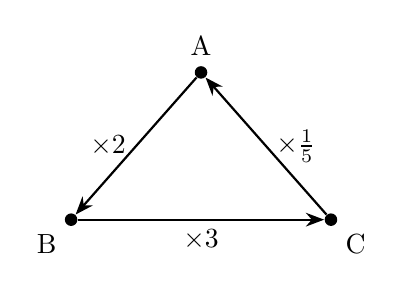
\begin{tikzpicture}[>=Stealth,scale=1.1]
\node[circle,fill,inner sep=1.6pt,label=above:A] (A) at (0,1.7) {};
\node[circle,fill,inner sep=1.6pt,label=below left:B] (B) at (-1.5,0) {};
\node[circle,fill,inner sep=1.6pt,label=below right:C] (C) at (1.5,0) {};
\draw[->,thick] (A) -- node[left] {$\times2$} (B);
\draw[->,thick] (B) -- node[below] {$\times3$} (C);
\draw[->,thick] (C) -- node[right] {$\times\frac15$} (A);
\end{tikzpicture}

{\small Around the loop the factor is $6/5$.}
\end{center}
If we look for measurements $x_A,x_B,x_C$ consistent with this table, the three equations give $x_A=\frac65x_A$, so
$x_A=0$. \emph{The only consistent measurement is $0$.} If the last entry is changed to $\frac16$, the product around the
loop becomes $1$, and every $x_A$ extends to exactly one consistent measurement.

There is a second point. To convert a value in A into a value in C, going through B multiplies by $6$, while reversing the
conversion ``from C to A'' multiplies by $5$. \emph{Unless we say which route was used, the answer is not determined.}

\subsection{The angle on a circle}
Mochizuki explains, with the analogy of manifolds, that omitting labels produces apparent contradictions.

\srcquote{\q{(This example may, roughly speaking, be thought of as a sort of generalization of the example discussed in
(LbEx1).) Consider the theory of (topological or differential) \textbf{manifolds} of dimension $n$, for $n$ a positive
integer. Manifolds (of dimension $n$) are, by definition, collections of \emph{distinct copies} --- i.e., copies equipped
with \textbf{distinct labels} --- of ($n$-dimensional) \emph{Euclidean space} glued together by means of various
\emph{gluing isomorphisms}. In particular, it is quite possible that the use of \textbf{numerous distinct copies of
Euclidean space} in this theory might impress a newcomer to this theory (such as a student) as being entirely
\textbf{superfluous}. Such a newcomer might feel motivated to attempt to achieve a \textbf{`dramatic simplification'} of
this theory by \textbf{identifying} these copies of Euclidean space with one another and hence to assert that the
geometry of \emph{arbitrary} (topological or differential) \emph{manifolds} (of dimension $n$) may be
\textbf{`reduced'} to the geometry of ($n$-dimensional) \emph{Euclidean space}.} \dots\par
\q{If one \textbf{identifies} these \textbf{distinct copies of Euclidean space} that appear in the theory of (topological or
differential) manifolds with one another, then it is easy to obtain a \emph{`contradiction'}. Such a `contradiction' may,
of course, be \emph{misinterpreted} as an \textbf{`internal contradiction'} in the theory of (topological or
differential) manifolds. In fact, however, there is \textbf{no `internal contradiction'} in the theory of (topological or
differential) manifolds; the apparent `internal contradiction' is nothing more than a superficial consequence of the
\textbf{erroneous operation} of \emph{omitting the labels} used to distinguish the distinct copies of Euclidean
space.}}{\cite[\S14, (LbEx5)]{R18}}

\begin{example}[Two charts of the circle]
Cover the circle by two coordinate charts. Let $U_1$ be the circle minus the point $(1,0)$, with the angle
$\theta_1\in(0,2\pi)$ as coordinate, and $U_2$ the circle minus $(-1,0)$, with the angle $\theta_2\in(-\pi,\pi)$. The
overlap has two parts, the upper and the lower half; on the upper half $\theta_2=\theta_1$, and on the lower half
$\theta_2=\theta_1-2\pi$.
\end{example}
The two coordinates are two ``copies of the real line''. The two parts of the overlap give two different identifications,
the identity and the translation by $-2\pi$. Going once around the circle shifts the angle by $2\pi$, so there is no
continuous angle function on the whole circle that is consistent with both charts. If the two copies are not
distinguished and are regarded as one real line, the apparent contradiction ``$\theta=\theta+2\pi$'' appears. The circle
is the simplest instance of Mochizuki's analogy.

In Example~2.1 a value is \emph{multiplied} by a factor around the loop; in Example~2.2 it is \emph{shifted} by an
amount. From now on we treat the first form (scaling), which is the one that appears in the IUT dispute.

\section{Indexed identifications}\label{s:indexed}

\subsection{Containers and identifications}
\begin{definition}[Containers]
A copy of the real line carrying a label $\alpha$ is written $\R_\alpha$ and called a \emph{container}. An element of
$\R_\alpha$ is thought of as ``a value measured in the units of $\alpha$''. Containers with different labels are treated
as different objects, even though as sets they are the same $\R$.
\end{definition}

\srcquote{A global realified Frobenioid \q{simply amounts to a collection of ordered 1-dimensional $\mathbb{R}$-vector
spaces $\mathbb{R}_v$ parametrized by the places $v$ of $k$, together with a subspace} $D_0$ of their direct sum \q{of
codimension 1}, subject to a normalization by the local degrees; and \q{These considerations show that the category of
global realified Frobenioids is equivalent to the category of ordered 1-dimensional $\mathbb{R}$-vector
spaces.}}{\cite[\S2.1.4]{SS}}

\tagH\ An ordered one-dimensional real vector space can be identified with $\R$ once a unit (a positive basis vector) is
chosen; changing the unit multiplies values by a positive real number. In this note we use from the start containers
with a chosen unit, that is, labelled copies of $\R$.

\begin{definition}[Identifications]\tagR
\known{\cite[Prop.~2.4\,(ii)]{Ur}, \cite[\S2.1.4]{SS}}
An \emph{identification} from the container $\R_\alpha$ to $\R_\beta$ is a map $f(x)=\lambda x$ given by multiplication
by a positive number $\lambda$; we call $\lambda=\lambda_f$ the \emph{scale} of $f$. For $x\in\R_\alpha$ and
$y\in\R_\beta$ with $y=f(x)$ we write
\[x\approx_f y\]
and read it as ``$x$ and $y$ are identified by $f$''.
\end{definition}

\subsection{Four rules}
\begin{proposition}[Rules]\tagP\tagR
\known{\cite[Prop.~2.4]{Ur}; for (R4), \cite[footnote~8]{SS} and \cite[Cor.~3.12]{IUT3}}
\begin{enumerate}[label=(R\arabic*)]
\item \emph{Identity and inverse.} $x\approx_{\id}x$. If $x\approx_f y$, then $y\approx_{f^{-1}}x$, and
$\lambda_{f^{-1}}=1/\lambda_f$.
\item \emph{Composition.} If $x\approx_f y$ and $y\approx_g z$, then $x\approx_{g\circ f}z$, and
$\lambda_{g\circ f}=\lambda_g\lambda_f$.
\item \emph{Action on numbers.} If $x\approx_f y$, then $y=\lambda_f x$; in particular the value itself changes under an
identification. Only quantities that are unchanged by all identifications (\emph{invariants}) may be transported without
naming the identification.
\item \emph{Sets of indices.} For a set $S$ of identifications we write $x\approx_S y$ for ``$x\approx_f y$ for some
$f\in S$'', and call
\[S(x):=\{\,f(x)\mid f\in S\,\}\]
the set of \emph{possible images} of $x$. The composite of two such sets is
$T\circ S:=\{\,g\circ f\mid f\in S,\ g\in T\,\}$.
\end{enumerate}
\end{proposition}
\begin{proof}
(R1) and (R2) follow from $f^{-1}(y)=y/\lambda_f$ and $g(f(x))=\lambda_g\lambda_f\,x$. (R3) and (R4) follow directly from
the definitions.
\end{proof}

\begin{definition}[Comparison with an error]\tagR
\known{\cite[\S2.2]{SS} (blurring)}
For $E\ge0$ and real numbers $a,b$ we write $a\le_E b$ for $a\le b+E$.
\end{definition}

\begin{remark}\tagH\ 
The ordinary equality sign corresponds to the case in which (R1) and (R2) hold and there is always only one
identification. The indexed symbol keeps in the formula which identification was used. If any of the four rules is
dropped, the index becomes decoration; for example, if (R3) is ignored and values are transported without the index, we
are in the situation of Proposition~\ref{p:sign}.
\end{remark}

\subsection{What remains when the index is dropped}
\begin{proposition}\label{p:sign}\tagP\ {\footnotesize (elementary)}\par
Write $x\approx y$, dropping the index, for ``$x\approx_f y$ for some identification $f$''. Then $x\approx y$ holds if and
only if $x$ and $y$ have the same sign (both positive, both $0$, or both negative).
\end{proposition}
\begin{proof}
Since scales are positive, identifications preserve signs. Conversely, if both are positive or both negative, take
$\lambda=y/x>0$; then $f(x)=y$. If both are $0$, any $f$ will do.
\end{proof}

\begin{proposition}[Invariants]\label{p:inv}\tagP\ {\footnotesize (elementary)}\par
For two values $x,x'$ in one container, with $x\neq0$, the ratio $x'/x$ and the order relation $x\le x'$ do not change
under any identification. The values themselves, their absolute values and their differences are multiplied by
$\lambda_f$.
\end{proposition}
\begin{proof}
$f(x')/f(x)=\lambda_f x'/(\lambda_f x)=x'/x$; since $\lambda_f>0$, the order is preserved; and
$f(x')-f(x)=\lambda_f(x'-x)$.
\end{proof}

\begin{remark}\tagH\ 
Comparisons inside one container do not depend on units. To compare values in different containers as numbers, one must
name an identification (by Proposition~\ref{p:sign}, without a name only the sign survives). In the usual way of writing,
this naming is hidden inside ``comparing them as real numbers''. Mochizuki makes the same point with the logarithm.
\end{remark}

\srcquote{\q{Thus, the substantial discomfort that some high-school students encounter in accepting the notion of a
logarithm may be understood as a difficulty in accepting the \textbf{identification} of the underlying additive monoid of
the topological field $\mathbb{R}$ that contains the multiplicative monoid $\mathbb{R}_{>0}$ in the \textbf{domain} of
$\log$ with the underlying additive monoid of the topological field $\mathbb{R}$ that appears in the \textbf{codomain} of
$\log$ on the grounds that the map $\log$ is \textbf{not compatible} with [i.e., does not arise from a ring homomorphism
between] the \textbf{ring structures} in its domain and codomain. Here, we recall that this identification is typically
`taken for granted' or `regarded as not requiring any justification' in discussions concerning the natural logarithm on
positive real numbers.}}{\cite[\S3.11\,(ii)]{Alien}}

\section{Segment, loop and universal cover}\label{s:graphs}

\subsection{Diagrams and consistent values}
\begin{definition}[Diagrams]\tagR
\known{\cite[(LbEx1)]{R18}, \cite{Ur}}
A \emph{diagram} is a finite graph with a container $\R_v$ at each vertex $v$ and an identification
$f_e:\R_v\to\R_w$ on each edge $e$ from $v$ to $w$. A family of values $(x_v)_v$ is \emph{consistent} if
$x_v\approx_{f_e}x_w$ for every edge $e:v\to w$. For a closed path $\gamma$, which traverses edges forwards or
backwards and returns to its starting vertex, the product of the scales of its edges (the reciprocal for an edge
traversed backwards) is called the \emph{monodromy} of $\gamma$ and written $\lambda(\gamma)$.
\end{definition}

\begin{proposition}\label{p:graph}\tagP\tagR
\known{\cite{MO} (coverings are classified by the fundamental group), \cite[(LbEx1)]{R18}}
Suppose the graph of a diagram is connected.
\begin{enumerate}[label=(\roman*)]
\item If the graph has no cycles (it is a tree), then for every vertex $v_0$ and every $x_0\in\R_{v_0}$ there is exactly
one consistent family of values with $x_{v_0}=x_0$.
\item If some closed path $\gamma$ through $v_0$ has $\lambda(\gamma)\ne1$, then every consistent family of values is $0$
at every vertex.
\item A consistent family of values that is not identically $0$ exists if and only if every closed path has
monodromy~$1$.
\end{enumerate}
\end{proposition}
\begin{proof}
(i) In a tree there is exactly one path from $v_0$ to each vertex; put at each vertex the transport of $x_0$ along that
path, and there is no other choice.
(ii) Transporting $x_{v_0}$ once around $\gamma$ gives $\lambda(\gamma)x_{v_0}$, which must equal $x_{v_0}$; hence
$(\lambda(\gamma)-1)x_{v_0}=0$ and $x_{v_0}=0$. Since the graph is connected, the value at every other vertex is the
transport of $0$, that is $0$.
(iii) If a family is not identically $0$, then by (ii) every closed path has monodromy $1$. Conversely, if every closed
path has monodromy $1$, choose a spanning tree and put values by (i) starting from some $x_0\ne0$; for an edge $e:v\to w$
outside the tree, the closed path formed by $e$ and the tree path has monodromy $1$, so $x_w=f_e(x_v)$.
\end{proof}
Example~2.1 is a triangular diagram whose monodromy around the loop is $6/5$; by Proposition~\ref{p:graph}\,(ii) the only
consistent value is $0$.
\companion{\cite[Props.~3.4 and 3.8]{Ur}}

\subsection{Mochizuki's three graphs}
\srcquote{\q{One considers the \emph{(`line segment') graph} $\Gamma_{\mathrm{seg}}$ \dots{} given by \emph{two vertices}
joined via a \emph{single edge}. Write $\Gamma_{\mathrm{loop}}$ for the \emph{(`loop') graph} obtained from
$\Gamma_{\mathrm{seg}}$ by identifying the \emph{two distinct vertices} of $\Gamma_{\mathrm{seg}}$ --- i.e., which may be
thought of as \emph{distinct labels} --- to a \emph{single vertex}. \dots{} situations where some sort of
\textbf{`parallel transport'} or \textbf{`analytic continuation'} along the \textbf{loop} of $\Gamma_{\mathrm{loop}}$ gives
rise to some sort of \textbf{nontrivial monodromy operator}. This sort of nontrivial monodromy may be \textbf{resolved}
\dots{} \emph{by working over $\Gamma_{\mathrm{seg}}$ as opposed to $\Gamma_{\mathrm{loop}}$}. When, moreover, one wishes
to distinguish situations that arise \emph{prior to} and \emph{subsequent to} multiple applications of the monodromy
operator, it is natural to consider the \emph{universal covering} $\Gamma_{\mathrm{uni}}$ \dots{} of
$\Gamma_{\mathrm{loop}}$} \dots\par
\q{one may understand the \textbf{incompatibility} of the \textbf{\boldmath$\Theta$-link} \dots{} with \textbf{arithmetic
degrees} \dots{} as a sort of \textbf{nontrivial monodromy} around the \textbf{loop} \dots{} that arises as soon as one
\emph{identifies} the \emph{domain} and \emph{codomain} of the $\Theta$-link --- an incompatibility \dots{} that is in fact
\textbf{avoided} in IUTch \dots{} precisely by \textbf{distinguishing} \emph{the (ring structures in the) domain and
codomain of the $\Theta$-link}, i.e., by working with `$\Gamma_{\mathrm{seg}}$', and then applying the \textbf{multiradial
algorithms} of IUTch to obtain an alternative way to \textbf{compute this nontrivial monodromy}}}{\cite[\S14, (LbEx1)]{R18}}

\begin{center}
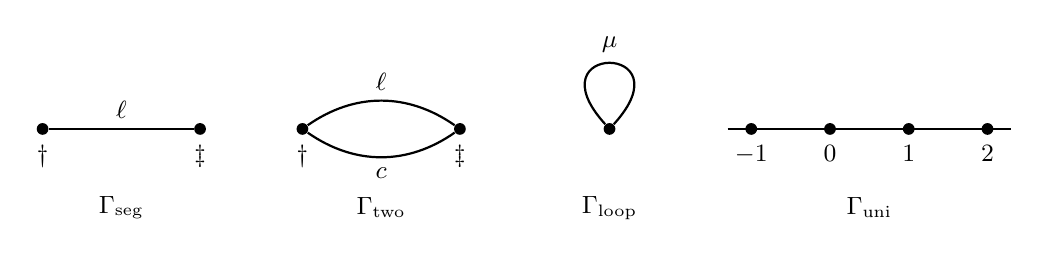
\begin{tikzpicture}[>=Stealth,every node/.style={font=\small}]
\begin{scope}
\node[circle,fill,inner sep=1.5pt,label=below:$\dagger$] (a) at (0,0) {};
\node[circle,fill,inner sep=1.5pt,label=below:$\ddagger$] (b) at (2,0) {};
\draw[thick] (a) -- node[above] {$\ell$} (b);
\node at (1,-1) {$\Gseg$};
\end{scope}
\begin{scope}[xshift=3.3cm]
\node[circle,fill,inner sep=1.5pt,label=below:$\dagger$] (a) at (0,0) {};
\node[circle,fill,inner sep=1.5pt,label=below:$\ddagger$] (b) at (2,0) {};
\draw[thick] (a) to[bend left=35] node[above] {$\ell$} (b);
\draw[thick] (a) to[bend right=35] node[below] {$c$} (b);
\node at (1,-1) {$\Gtwo$};
\end{scope}
\begin{scope}[xshift=6.6cm]
\node[circle,fill,inner sep=1.5pt] (a) at (0.6,0) {};
\draw[thick] (a) .. controls (-0.4,1.1) and (1.6,1.1) .. node[above] {$\mu$} (a);
\node at (0.6,-1) {$\Gloop$};
\end{scope}
\begin{scope}[xshift=9cm]
\draw[thick] (-0.3,0) -- (3.3,0);
\foreach \x/\n in {0/-1,1/0,2/1,3/2} {\node[circle,fill,inner sep=1.5pt,label=below:$\n$] at (\x,0) {};}
\node at (1.5,-1) {$\Guni$};
\end{scope}
\end{tikzpicture}
\end{center}

\tagH\ In terms of diagrams this reads as follows.
\begin{itemize}
\item \emph{Segment $\Gseg$.} The vertices $\dagger,\ddagger$ are joined by one edge $\ell$. There is no cycle, so values
are unconstrained (Proposition~\ref{p:graph}\,(i)).
\item \emph{Two paths $\Gtwo$.} The same two vertices are joined by two edges $\ell$ and $c$. The closed path that goes
from $\dagger$ to $\ddagger$ along $\ell$ and back along $c$ reversed has monodromy $\lambda_c^{-1}\lambda_\ell$.
\item \emph{Loop $\Gloop$.} Merging $\dagger$ and $\ddagger$ into one vertex along the edge $c$ turns the remaining edge
$\ell$ into a loop, with scale $\lambda_\mu=\lambda_c^{-1}\lambda_\ell$ of $\mu:=c^{-1}\circ\ell$. If this is not $1$,
the only value is $0$ (Proposition~\ref{p:graph}\,(ii)).
\item \emph{Universal cover $\Guni$.} Label the vertices by integers $n$ and put $\mu$ on each edge from $n$ to $n+1$.
There is no cycle, so every $x_0$ determines exactly one consistent family $x_n=\lambda_\mu^{\,n}x_0$
(Proposition~\ref{p:graph}\,(i) and Exercise~4). The label $n$ remembers how many times one has gone around.
\end{itemize}
\companion{\cite[Props.~3.4--3.9]{Ur}}

\subsection{The loop with the labels dropped}
\begin{proposition}\label{p:orbit}\tagP\tagR
\known{\cite[Remark~3.11.1\,(vii),\,(viii)]{IUT3}}
Let $0<m<1$ and $x_0<0$, and put
\[O:=\{\,m^nx_0\mid n\in\Z\,\}.\]
This is the family of values on the universal cover with the labels $n$ dropped, that is, the set of possible images of
$x_0$ under $\{\mu^n\mid n\in\Z\}$ (with $\lambda_\mu=m$). Then $\sup O=0$ (there is no maximum) and $\inf O=-\infty$.
Hence the smallest interval containing $O$ is $(-\infty,0)$, and for a negative number $a$ the statement ``$a\le\sup O$''
always holds and says nothing.
\end{proposition}
\begin{proof}
Every element is negative; $m^nx_0\to0$ as $n\to+\infty$ and $m^nx_0\to-\infty$ as $n\to-\infty$.
\end{proof}

\srcquote{\q{one is led [at least in the absence of more sophisticated machinery!] to regard
`$\underline{\underline{q}}$' as being \textbf{only well-defined up to possible confusion with
`\boldmath$\underline{\underline{q}}^{\lambda^n}$'}, for some indeterminate $n\in\mathbb{Z}$. That is to say, in summary,
this approach gives rise to a sort of \textbf{`uninteresting/trivial multiradial representation} of
`$\underline{\underline{q}}^{\lambda}$' via}
\[\text{``}\{\underline{\underline{q}}^{\lambda^n}\}_{n\in\mathbb{Z}}\text{''}\]
\dots\par
\q{this `trivial multiradial representation' is \textbf{useless} from the point of view of applications such as the
log-volume estimates given in Corollary 3.12 below \dots{} for the following reasons: This \textbf{`trivial multiradial
representation \boldmath$\{\underline{\underline{q}}^{\lambda^n}\}_{n\in\mathbb{Z}}$'} is obtained by
\textperiodcentered\ allowing for \textbf{indeterminacies} in the \textbf{value group} portion [i.e.,
`$\underline{\underline{q}}^{\mathbb{Z}}$'] of the data under consideration, \dots}\par
\q{By contrast, the \emph{log-volume estimates} of Corollary 3.12 below rely, in an essential way, on the fact that in the
\textbf{multiradial construction algorithm} of Theorem 3.11: \textperiodcentered\ the \textbf{value group} portions of the
data under consideration \dots{} are held \textbf{rigid} [i.e., are not subject to indeterminacies],
\textperiodcentered\ while the \textbf{unit group} portions of the data under consideration \dots{} are subject to the
\textbf{indeterminacies} (Ind1), (Ind2), (Ind3); \dots}}{\cite[Remark~3.11.1\,(vii),\,(viii)]{IUT3}}

\tagH\ The log-volume of $\qq^{\lambda^n}$ is $\lambda^n\log\qq$, so the source's $\{\qq^{\lambda^n}\}_{n\in\Z}$
corresponds to the orbit of Proposition~\ref{p:orbit}. If the labels are dropped and one may go around the loop any
number of times, the comparison becomes empty.
\companion{\cite[Thm.~5.5]{Ur}}

\section{The \texorpdfstring{$\Theta$}{Theta}-link and two paths}\label{s:theta}

\subsection{The model}
\begin{setup}[The model]\label{setup}\tagR
\known{\cite[\S2.1.4, \S2.2]{SS}, \cite[\S7.1, \S10.2]{LANA}}
Consider the following data.
\begin{enumerate}[label=(\alph*)]
\item Containers $\R_\dagger$ and $\R_\ddagger$ for the values of log-volumes on the domain ($\Theta$ side) and on the
codomain ($q$ side) of the $\Theta$-link.
\item Two identifications $\ell,c:\R_\dagger\to\R_\ddagger$: $\ell$ is the $\Theta$-link (it sends the $\Theta$-pilot
to the $q$-pilot), and $c$ is the natural identification that comes from both sides arising from the same curve.
\item $b\in\R_\dagger$ is the log-volume of the $\Theta$-pilot and $a\in\R_\ddagger$ that of the $q$-pilot. The
$\Theta$-link gives $b\approx_\ell a$.
\item Units are chosen so that the scale of $c$ is $1$. Put $Q:=|\log q|>0$, $a=-Q$ and $b=-kQ$, where $k$ is the mean of
$j^2$ over $j=1,\dots,l^*$ with $l^*=(l-1)/2$:
\[k:=\frac{1}{l^*}\sum_{j=1}^{l^*}j^2=\frac{l(l+1)}{12}\]
(Exercise~3). Then $\lambda_\ell=1/k$ and $\lambda_c=1$.
\item An error $E\ge0$: a single number standing for the error produced by the indeterminacies of the multiradial
algorithm.
\end{enumerate}
\end{setup}
\begin{remark}\tagH\ 
The identification $c$ in (b) corresponds to the identification that Scholze--Stix make by \q{using the natural isomorphisms
$\mathbb{R}_{\odot,\Theta}\cong\mathbb{R}_{\odot,q}\cong\mathbb{R}$}~\cite[\S2.2]{SS}. Mochizuki's
position is not to use it as an identification (Section~\ref{s:toy}); in the model, whether it is used can be read off
from the indices. For a prime $l\ge5$ we have $k-1=(l+4)(l-3)/12>0$. Finer normalizations (such as the $2l$-th root of
$q$) are omitted in the model. This is the same model as~\cite[Setup~5.1]{Ur}.
\end{remark}

\subsection{The three options of Scholze--Stix}
\begin{proposition}\label{p:three}\tagP\tagR
\known{\cite[\S2.2]{SS}}
In Setup~\ref{setup}:
\begin{enumerate}[label=(\alph*)]
\item \emph{Use both.} If both $\ell$ and $c$ are used as identifications (the diagram $\Gtwo$) and values are required to
be consistent, the only value is $0$. Since $a=-Q\ne0$, this requirement is incompatible with the $\Theta$-link.
\item \emph{Make them one.} If $\ell$ and $c$ are made the same identification ($\lambda_\ell=\lambda_c$), then $k=1$:
the factor $j^2$ is omitted. The comparison $a\le c(b)+E$ then reads $-Q\le-Q+E$, that is $0\le E$, and says nothing.
\item \emph{Blur.} If $k$ is kept and the results of transport along the two paths are compared up to an error $E$, that
is, if one asks for $\ell(b)\le_E c(b)$, this is equivalent to $(k-1)Q\le E$. Here $k-1=(l+4)(l-3)/12$ grows like $l^2$.
\end{enumerate}
\end{proposition}
\begin{proof}
(a) The closed path of $\Gtwo$ has monodromy $\lambda_c^{-1}\lambda_\ell=1/k\ne1$; apply
Proposition~\ref{p:graph}\,(ii).
(b) $1/k=\lambda_\ell=\lambda_c=1$ gives $k=1$; then $b=-Q$ and $c(b)=-Q$.
(c) Since $\ell(b)=a=-Q$ and $c(b)=-kQ$, the inequality $-Q\le-kQ+E$ is equivalent to $(k-1)Q\le E$.
\end{proof}

\srcquote{(a)~\q{However, it is clear that this will result in the whole diagram having monodromy $j^2$, i.e., being
inconsistent.}\par
(b)~\q{The conclusion of this discussion is that with consistent identifications of copies of real numbers, one must
\dots\ omit the scalars $j^2$ that appear, which leads to an empty inequality.}\par
(c)~\q{In particular, he claimed that up to the `blurring' given by certain indeterminacies the diagram does commute; it
seems to us that this statement means that the blurring must be by a factor of at least $\mathrm{O}(\ell^2)$ rendering the
inequality thus obtained useless.}}{\cite[\S2.2]{SS}; the labels (a), (b), (c), showing the correspondence with
Proposition~\ref{p:three}, are ours}

\tagH\ The factor of at least $\mathrm{O}(\ell^2)$ in (c) corresponds in the model to the factor $k=l(l+1)/12$ that moves
$b=-kQ$ to $a=-Q$, that is, to the added error $(k-1)Q$.
\companion{\cite[Thms.~5.2 and 5.3]{Ur}}

\subsection{The part that is not disputed}
\srcquote{(AD) \q{The correspondence that appears in the \textbf{\boldmath$\Theta$-link}
\[\{\underline{\underline{q}}^{j^2}\}\quad\mapsto\quad\underline{\underline{q}}\]
(where $j=1,\ldots,l^{\divideontimes}$) is, when considered within/relative to a \textbf{single hol.\ str.}, i.e., a
\textbf{single ring/scheme theory}, manifestly \textbf{incompatible/inconsistent} with computing \textbf{arithmetic
degrees}, unless one considers arithmetic degrees up to the \textbf{indeterminacy} \emph{given by possible multiplication
by factors `$j^2$'} (where $j=1,\ldots,l^{\divideontimes}$) --- an indeterminacy which then renders the computation
\emph{meaningless}.}\par
(IUAD) \q{There is \textbf{absolutely no dispute} whatsoever (between SS and HM) with respect to the validity of the
assertion (AD).}}{\cite[\S12, (AD), (IUAD)]{R18}}
\tagH\ Proposition~\ref{p:three}\,(a) corresponds to the first half of (AD) (inside a single ring theory the two are
incompatible), and Proposition~\ref{p:orbit} to the second half (introducing the indeterminacy makes the computation
meaningless). On this part there is, as Mochizuki says, no dispute.

\section{Mochizuki's elementary numerical model}\label{s:toy}

\subsection{Example 3.11.4}
\srcquote{\q{the overall general \emph{logical flow} of inter-universal Teichm\"uller theory --- i.e., starting from the
definition of the \emph{$\Theta$-link}, proceeding to the \emph{multiradial representation of the $\Theta$-pilot} [cf.\
[IUTchIII], Theorem 3.11], and finally, culminating in a \emph{final numerical estimate} [cf.\ [IUTchIII], Corollary
3.12] --- may be represented by means of \emph{real numbers} $A, B \in \mathbb{R}_{>0}$ and $\epsilon, N \in \mathbb{R}$
such that $0 \leq \epsilon < 1$ in the following way:
\begin{itemize}
\item[$\cdot$] \textbf{\boldmath$\Theta$-link}:
\[\bigl(N \stackrel{\mathrm{def}}{=} -2B\bigr)\quad\wedge\quad\bigl(N \stackrel{\mathrm{def}}{=} -A\bigr);\]
\item[$\cdot$] \textbf{multiradial representation of the \boldmath$\Theta$-pilot}:
\[\bigl(N = -2A + \epsilon\bigr)\quad\wedge\quad\bigl(N = -A\bigr);\]
\item[$\cdot$] \textbf{final numerical estimate}:
\[-2A + \epsilon = -A, \text{ hence } A = \epsilon, \text{ i.e., } A < 1.\]
\end{itemize}
Thus, the \emph{$\Theta$-link} \dots{} and \emph{multiradial representation of the $\Theta$-pilot} \dots{} are
\emph{meaningful/nontrivial} precisely because of the \textbf{logical relator} `$\wedge$', whose use obligates one, in the
definition of the $\Theta$-link, to consider \emph{a priori} \textbf{distinct} real numbers $A$, $B$} \dots\par
\q{the use of \emph{distinct} real numbers $A$, $B$ in the definition of the `$\vee$' version of $\Theta$-link seems
\emph{entirely superfluous} \dots. This motivates one to \emph{identify} $A$ and $B$ --- i.e., to suppose \emph{`for the
sake of simplicity'} that $A = B$ --- which then has the effect of rendering the definition of the original `$\wedge$'
version of the $\Theta$-link \emph{invalid/self-contradictory}}}{\cite[Example~3.11.4]{Alien}}

\subsection{Reading it with indices}
\tagH\ The ingredients of Example~3.11.4 correspond to the notation of Setup~\ref{setup} as follows.

\begin{center}\small
\begin{tabularx}{\linewidth}{@{}>{\raggedright\arraybackslash}X>{\raggedright\arraybackslash}X@{}}
\toprule
Example 3.11.4 & This note (Setup~\ref{setup})\\
\midrule
A priori distinct positive reals $A,B$ & The same size measured in the units of the $q$ side ($\ddagger$) and of the
$\Theta$ side ($\dagger$); without $c$ the two cannot be compared\\
The factor $2$ & The mean $k$ of $j^2$\\
$(N\stackrel{\mathrm{def}}{=}-2B)\wedge(N\stackrel{\mathrm{def}}{=}-A)$ (the $\Theta$-link) & $b\approx_\ell a$: one
object is described as $b$ on the $\Theta$ side (in the example $-2B$) and as $a=-A$ on the $q$ side\\
Identifying $A=B$ ``for simplicity'' & Using $c$ as an identification as it stands and collecting everything into one
number $N$; by Proposition~\ref{p:three}\,(a) the only value is $0$ (a self-contradiction)\\
$(N=-2A+\epsilon)\wedge(N=-A)$ (the multiradial representation) & $a=c(b)+\varepsilon$: the results of transport along
the two paths agree up to the error $\varepsilon$\\
$A=\epsilon$, $A<1$ (the final estimate) & $(k-1)Q=\varepsilon$, $Q<1/(k-1)$\\
\bottomrule
\end{tabularx}
\end{center}

\begin{proposition}\label{p:toy}\tagP\tagR
\known{\cite[Example~3.11.4]{Alien}}
In Setup~\ref{setup}, assume $k>1$.
\begin{enumerate}[label=(\roman*)]
\item If $a=c(b)+\varepsilon$ with $0\le\varepsilon<1$, then $(k-1)Q=\varepsilon$, and hence $Q<1/(k-1)$. For $k=2$ this
gives $Q=\varepsilon<1$, the same formula as the final estimate $A=\epsilon<1$ of Example~3.11.4.
\item $\ell(b)\le_E c(b)$ is equivalent to $(k-1)Q\le E$.
\end{enumerate}
\end{proposition}
\begin{proof}
Substitute $\ell(b)=a=-Q$ and $c(b)=-kQ$: (i) $-Q=-kQ+\varepsilon$; (ii) Proposition~\ref{p:three}\,(c).
\end{proof}

\subsection{The content lies in the license}
\srcquote{\q{Put another way, this algorithm allows one to} \dots\par
\q{$(4^{\mathrm{cld}})$ construct a \textbf{closed loop} --- i.e., from a given \emph{input data}
[\emph{$q$-intertwined}!] $\mathcal{F}^{\Vdash\blacktriangleright\times\boldsymbol{\mu}}$-prime-strip back to the given
\emph{input data} [\emph{$q$-intertwined}!] $\mathcal{F}^{\Vdash\blacktriangleright\times\boldsymbol{\mu}}$-prime-strip
--- whose \emph{output data} consists of the \emph{$\Theta$-intertwining} [up to suitable \emph{indeterminacies}] on this
single given input data [\emph{$q$-intertwined}!]
$\mathcal{F}^{\Vdash\blacktriangleright\times\boldsymbol{\mu}}$-prime-strip [cf.\ the discussion of the final portion of
[IUTchIII], Remark 3.9.5, (ix)]. Here, we note that it is precisely this \emph{closed} nature of the loop that allows one
to derive \dots{} \emph{nontrivial consequences} \dots{} from the \emph{multiradial representation of the
$\Theta$-pilot}.}}{\cite[\S3.11\,(v)]{Alien}}

\tagH\ In the model this closed path goes from $\ddagger$ back to $\dagger$ along $c$ reversed and returns to $\ddagger$
along $\ell$. Its monodromy is $1/k$, not $1$ (Proposition~\ref{p:three}\,(a)). That the output data is obtained \q{up to suitable
\emph{indeterminacies}} can be read as saying that the results of transport along the two paths agree within the error $E$,
that is, $\ell(b)\le_E c(b)$.

\begin{remark}[What is disputed]\tagH\ 
In Example~3.11.4 the two descriptions determine $\epsilon=(k-1)A$ exactly ($\epsilon=A$ for $k=2$). So ``$\epsilon$ is
small'' and ``$A$ is small'' are the same statement. When Mochizuki writes that, once one is equipped with this license, the
derivation of the bounds on heights is an essentially formal matter, this is accurate in that sense: the content lies in
the license itself.

What is disputed is whether Theorem~3.11 of IUT~III (the multiradial algorithm) provides the license with a small error
independently of the conclusion. Mochizuki says that it does; Scholze--Stix say that the blurring must be by a factor of at
least $O(l^2)$, which renders the inequality thus obtained useless. The model is consistent with both: one can build
models with $E\ge(k-1)Q$ and models with $E<(k-1)Q$. Which holds for the actual construction is outside the model.
\end{remark}
\companion{\cite[Thms.~5.3 and 5.7]{Ur}}

\section{Corollary 3.12 and the upper bound of IV}\label{s:cor}
\srcquote{Corollary~3.12: write $-|\log(\Th)|\in\R\cup\{+\infty\}$ for the procession-normalized mono-analytic
log-volume of the holomorphic hull of the union of the possible images of a $\Theta$-pilot object in the multiradial
representation of Theorem~3.11, which is regarded as subject to the indeterminacies (Ind1), (Ind2), (Ind3); and write
$-|\log(\qq)|\in\R$ for the procession-normalized mono-analytic log-volume of the image of a $q$-pilot object, which is not
regarded as subject to these indeterminacies. Here $|\log(\qq)|>0$. Then \q{it holds that
$-|\log(\underline{\underline{\Theta}})|\in\mathbb{R}$, and
$-|\log(\underline{\underline{\Theta}})|\geq-|\log(\underline{\underline{q}})|$}.}{\cite[Cor.~3.12]{IUT3}}

\begin{proposition}\label{p:cor}\tagP\tagR
\known{\cite[\S2.2]{SS}}
In Setup~\ref{setup}, let $-|\log\Theta|:=c(b)+E$ be the value of the hull of the possible images of the $\Theta$-pilot,
computed through $c$. Then the inequality $-|\log\Theta|\ge-|\log q|$ of Corollary~3.12 is equivalent to
$\ell(b)\le_E c(b)$, and hence to $(k-1)Q\le E$.
\end{proposition}
\begin{proof}
Since $-|\log q|=a=\ell(b)$, the inequality reads $\ell(b)\le c(b)+E$; now apply Proposition~\ref{p:toy}\,(ii).
\end{proof}

\begin{corollary}\label{c:height}\tagP\tagR
\known{\cite[Introduction]{Alien}, \cite[Thm.~1.10]{IUT4}}
If IV bounds the error from above by $E\le C$, with $C$ independent of $Q$, then Corollary~3.12 implies $Q\le C/(k-1)$.
\end{corollary}
\begin{proof}
$(k-1)Q\le E\le C$ and $k-1>0$.
\end{proof}

\begin{remark}\tagH\ 
(i) For $k=1$ (omitting $j^2$) we get $k-1=0$ and nothing follows. The information, an upper bound for $Q$, comes from
$k>1$, that is, from $j^2$; and $k>1$ is also what produces the monodromy $1/k\ne1$ of the two paths. The content of
Corollary~3.12 and the difficulty of the dispute come from the same $j^2$.

(ii) The actual estimate of IV~\cite[Thm.~1.10]{IUT4} contains terms such as differents and conductors, and $C$ depends on
$l$. The model keeps only the shape. $Q$ is the size of $q$, and its upper bound has the shape of a height inequality (an
inequality of abc type).
\end{remark}
\companion{\cite[Cor.~5.4]{Ur}}

\section{The two positions in one table}\label{s:table}
\tagH\ The following table summarizes the above in the notation of Setup~\ref{setup}.

\begin{center}\small
\begin{tabularx}{\linewidth}{@{}>{\raggedright\arraybackslash}p{2.3cm}>{\raggedright\arraybackslash}X>{\raggedright\arraybackslash}X>{\raggedright\arraybackslash}X@{}}
\toprule
& Scholze--Stix \cite[\S2.2]{SS} & Mochizuki \cite{R18,Alien} & Common ground\\
\midrule
Identifications used & Both $\ell$ and $c$, consistently & Only the $\Theta$-link $\ell$; $c$ is recovered with an
error by the multiradial algorithm & Using both $\ell$ and $c$ as they stand leads to a contradiction ((AD), (IUAD);
Prop.~\ref{p:three}\,(a))\\
Graph & $\Gtwo$ (with a cycle) & $\Gseg$ (a segment); $\Guni$ if the number of turns is to be distinguished & If the
monodromy of a cycle is not $1$, the only consistent value is $0$ (Prop.~\ref{p:graph})\\
Reading of Cor.~3.12 & Omitting $j^2$ gives $0\le E$, which is empty; keeping it needs an error of at least $(k-1)Q$,
which is useless & From the license with a small error, the height bound follows formally & In the model,
Cor.~3.12 $\Leftrightarrow(k-1)Q\le E$ (Prop.~\ref{p:cor})\\
The decisive point & The error cannot be made small & Theorem~3.11 provides a small error & The decisive point is the
size of the error $E$ (its value lies outside the model)\\
\bottomrule
\end{tabularx}
\end{center}

\section{One level down: presented reals}\label{s:down}
\srcquote{\q{The theorem is proved over \emph{presented} reals---regular sequences of rationals with Bishop
equality---\dots\ rather than for an abstract real-number object.}}{\cite[Abstract]{U}}

In his formalization of presented reals~\cite{U}, the author treated real numbers through presentations that carry
witnesses of convergence. Two presentations of the same real number are related by a proposition, namely whether they are
equal as real numbers. \tagH\ In the language of this note, in the container reached after forgetting presentations,
the scale of every identification is $1$. Then every closed path has monodromy $1$, and the obstruction of
Proposition~\ref{p:graph}\,(ii) does not occur (Exercise~9). Forgetting a presentation loses only the presentation, and a
forgotten witness can be recovered without any choice principle when there is a decidable search.

\srcquote{\q{In Lean, a statement in \texttt{Prop} is proof-irrelevant, and an arbitrary witness hidden in a
\texttt{Prop}-valued existential cannot in general be eliminated into \texttt{Type} (data can nevertheless be recomputed
when an independent decidable search produces a witness---Appendix~B.12)}}{\cite[\S7.2]{U}}

\tagH\ Presented reals correspond to the case in which all scales are $1$. The difficulty of IUT lies in the fact that an
identification of scale $1/k\ne1$ cannot be avoided. The relation with locators, and a formulation that treats both
levels in the single language of homotopy type theory, are left to~\cite[\S7]{Ur}.

\section{Summary}\label{s:sum}
\begin{itemize}
\item Written with indexed identifications, ``identify or not'' becomes a formula about which edges of which diagram are
used.
\item \emph{Agreed:} using consistently an identification that does not return to $1$ around a loop leaves only the value
$0$ (Props.~\ref{p:graph} and~\ref{p:three}\,(a); (AD), (IUAD)). If the labels are dropped and one may go around the loop
any number of times, the comparison becomes empty (Prop.~\ref{p:orbit}; \cite[Remark~3.11.1\,(vii)]{IUT3}).
\item \emph{Disputed:} whether the comparison $\ell(b)\le_E c(b)$ of the two paths holds with an error small enough to be
compatible with the estimate $E\le C$ of IV. In the model this is equivalent to $(k-1)Q\le E$, which itself has the shape
of an upper bound for $Q$ (Prop.~\ref{p:cor} and Cor.~\ref{c:height}).
\item The model does not decide this question. What decides it is the size of the error produced by the actual
construction.
\end{itemize}

\section{Exercises}\label{s:ex}
\begin{exercise}
In the conversion table of Example~2.1, replace the last entry by $x_A=\frac16x_C$ and find all consistent measurements.
Explain, using Proposition~\ref{p:graph}, why with $\frac15$ the only one is $0$.
\end{exercise}
\begin{exercise}
Check, using (R1) and (R2), that the relation $x\approx y$ of Proposition~\ref{p:sign} is an equivalence relation
(reflexive, symmetric and transitive). How many equivalence classes are there?
\end{exercise}
\begin{exercise}
Using $\sum_{j=1}^{n}j^2=n(n+1)(2n+1)/6$, show that for $l^*=(l-1)/2$ one has $k=l(l+1)/12$ and $k-1=(l+4)(l-3)/12$. Compute
$k$ for $l=5,7,11,13$.
\end{exercise}
\begin{exercise}
For the diagram on the universal cover $\Guni$ with scale $\lambda$ on every edge, show that the consistent families of
values are exactly $x_n=\lambda^nx_0$.
\end{exercise}
\begin{exercise}
Check Proposition~\ref{p:orbit} for $m=\frac12$ and $x_0=-1$: list the elements of $O$ for $n=-2,\dots,2$.
\end{exercise}
\begin{exercise}
From the computation $-2A+\epsilon=-A$ of Example~3.11.4, derive $A=\epsilon$. What do you get if the factor $2$ is
replaced by $k$? What if the equality is replaced by the inequality $-A\le-kA+E$?
\end{exercise}
\begin{exercise}
In Corollary~\ref{c:height}, find the upper bound for $Q$ when $l=7$ and $C=1$. What happens when $k=1$?
\end{exercise}
\begin{exercise}
Which of the following are unchanged by all identifications: the sign; the absolute value; the ratio of two values in the
same container; the difference of two values in the same container?
\end{exercise}
\begin{exercise}[One level down]
Show that in a connected diagram all of whose edges have scale $1$, every closed path has monodromy $1$, and that a
consistent family of values can be built from any value at any vertex. This is the case of the presented reals of
Section~\ref{s:down}.
\end{exercise}

\subsection*{Answers}
\begin{enumerate}[label=\arabic*.]
\item $x_B=2x_A$ and $x_C=6x_A$, and $x_A=\frac16x_C$ holds for every $x_A$; the consistent measurements are exactly
$(t,2t,6t)$, $t\in\R$. With $\frac15$ the monodromy around the loop is $6/5\ne1$, so by Proposition~\ref{p:graph}\,(ii)
the only value is $0$.
\item Reflexivity comes from $\id$, symmetry from the inverse in (R1) and transitivity from the composite in (R2). There
are three classes: the negative numbers, $0$ and the positive numbers.
\item $k=(l^*+1)(2l^*+1)/6$ with $l^*+1=(l+1)/2$ and $2l^*+1=l$, so $k=l(l+1)/12$, and $k-1=(l^2+l-12)/12=(l+4)(l-3)/12$.
For $l=5,7,11,13$: $k=5/2,\ 14/3,\ 11,\ 91/6$.
\item The condition on the edge $n\to n+1$ is $x_{n+1}=\lambda x_n$. Induction gives $x_n=\lambda^nx_0$ for $n\ge0$, and
induction using $x_n=\lambda^{-1}x_{n+1}$ gives it for $n<0$. Conversely this family satisfies every condition.
\item For $n=-2,-1,0,1,2$: $-4,\ -2,\ -1,\ -\frac12,\ -\frac14$. As $n\to+\infty$ the elements approach $0$; as
$n\to-\infty$ they become arbitrarily small.
\item $A=\epsilon$. With the factor $k$: $(k-1)A=\epsilon$. With the inequality: $(k-1)A\le E$
(Proposition~\ref{p:toy}).
\item $k=14/3$ and $k-1=11/3$, so $Q\le3/11$. For $k=1$ the inequality reads $0\cdot Q\le E$ and gives no bound. In the
actual IV the constant $C$ also depends on $l$, so the model says nothing about the behaviour as $l$ grows.
\item The sign and the ratio (and the order relation) are unchanged. The absolute value and the difference are multiplied
by $\lambda_f$ (Proposition~\ref{p:inv}).
\item A product of scales equal to $1$ is $1$. As in the proof of Proposition~\ref{p:graph}\,(iii), put values along a
spanning tree; the conditions on the edges outside the tree then hold as well.
\end{enumerate}

\section*{Acknowledgements and use of AI}
The idea of this note (to write the shape of the dispute in undergraduate mathematics, with symbols for indexed
identifications in place of the equality sign) is the author's. Generative AI tools (large language models) were used
extensively, under the author's direction, in working out the propositions and their proofs and in the writing. The author
takes full responsibility for the contents of this note.

\begin{thebibliography}{IUT3}
\bibitem[Alien]{Alien}
Shinichi Mochizuki, \emph{The mathematics of mutually alien copies: from {G}aussian integrals to inter-universal
{T}eichm\"uller theory}, in: Inter-universal Teichm\"uller Theory Summit 2016, RIMS K\^oky\^uroku Bessatsu \textbf{B84}
(2021), 23--192.

\bibitem[IUT3]{IUT3}
Shinichi Mochizuki, \emph{Inter-universal {T}eichm\"uller theory {III}: canonical splittings of the log-theta-lattice},
Publ. Res. Inst. Math. Sci. \textbf{57} (2021), 403--626.

\bibitem[IUT4]{IUT4}
Shinichi Mochizuki, \emph{Inter-universal {T}eichm\"uller theory {IV}: log-volume computations and set-theoretic
foundations}, Publ. Res. Inst. Math. Sci. \textbf{57} (2021), 627--723.

\bibitem[LANA]{LANA}
Project LANA, \emph{Project LANA interim report on IUT theory}, last updated 20 July 2026.

\bibitem[MO]{MO}
Samuel Mimram and \'Emile Oleon, \emph{Classifying covering types in homotopy type theory}, in: 34th EACSL Annual Conference
on Computer Science Logic (CSL 2026), LIPIcs \textbf{363} (2026), 21:1--21:20,
\href{https://doi.org/10.4230/LIPIcs.CSL.2026.21}{doi:10.4230/LIPIcs.CSL.2026.21}; arXiv:2512.10064.

\bibitem[R18]{R18}
Shinichi Mochizuki, \emph{Report on discussions, held during the period March 15--20, 2018, concerning inter-universal
{T}eichm\"uller theory ({IUTch})}, February 2019.

\bibitem[SS]{SS}
Peter Scholze and Jakob Stix, \emph{Why abc is still a conjecture}, manuscript, 2018.

\bibitem[U]{U}
Toshihisa Urahigashi, \emph{A choice-free {L}ean formalization of {B}ishop--{C}heng dominated convergence over presented
reals}, manuscript, version 0.7.8, 5 September 2026, file \texttt{paper/paper.pdf} at tag \texttt{v0.7.8} of
\url{https://github.com/turahigashi/choicefree-bc-dct}; the Lean artifact is archived at Zenodo,
\href{https://doi.org/10.5281/zenodo.22333837}{doi:10.5281/zenodo.22333837}.

\bibitem[Ur]{Ur}
Toshihisa Urahigashi, \emph{Segment or loop? A homotopy-type-theoretic overview of the dispute over {C}orollary 3.12 of
inter-universal {T}eichm\"uller theory}, version 1.0.0, Zenodo, 4 November 2026, \href{https://doi.org/10.5281/zenodo.23931344}{doi:10.5281/zenodo.23931344}.
\end{thebibliography}
\end{document}
